\begin{otherlanguage}{slovene}
\chapter{Povzetek doktorskega dela}
\section{Uvod}
Fizika delcev je eden od stebrov fizike z mo"cnimi koreninami, ki segajo vse do za"cetka 20. stoletja. Natan"cni eksperimenti in preverljiva teorija so pokazali, da vesolje sestoji iz osnovnih delcev in nosilcev interakcij med njimi. Osnovne delce delimo na kvarke ($u$, $d$, $s$, $c$, $b$, $t$) in leptone, ki so nadaljnje razdeljeni na nabite leptone ($e$, $\mu$, $\tau$) in pa nevtrine ($\nu_e$, $\nu_\mu$, $\nu_\tau$). Nosilci treh (od "stirih) osnovnih interakcij, s katerimi se ukvarjamo na tem podro"cju, so fotoni ($\gamma$) za elektromagnetno, gluoni ($g$) za mo"cno in nabiti- ($W^\pm$) ter nevtralni ($Z^0$) bozoni za "sibko interakcijo. Vsi delci in njihovi zrcalni partnerji, antidelci (ozna"ceni z $~\bar {}~$), imajo maso, ki jim jo dolo"ca Higgsov bozon ($H$). Vse delce ter interakcije med njimi opisuje Standardni model, ki je osrednja teorija fizike visokih energij. Kvarke lahko zdru"zujemo v kombinacije oblike $q_1 q_2 q_3$ (hadroni) ali pa $q_1 \bar{q}_2$ (mezoni), kamor med prve uvr"s"camo tudi protone in nevtrone. Poleg omenjenih dolgo-"zive"cih delcev pa obstajajo tudi te"zji, manj stabilni delci, ki preko zgoraj na"stetih interakcij razpadajo v la"zje in stabilnej"se. Raziskovanje tak"snih procesov s pomo"cjo pospe"sevalnikov in trkalnikov nam danes omogo"ca spoznavanje zakonov vesolja vse do njegovega za"cetka.

Osrednji del doktorske disertacije predstavljajo meritve razpadov mezonov $B$, t.j. delcev, ki so sestavljeni iz te"zkega kvarka $b$ in enega od lahkih kvarkov $u$ ali $d$. Ena bolj presenetljivih lastnosti vesolja je kr"sitev simetrije $CP$, t.j. kombinacije simetrij konjugacije naboja ($C$) in prostorske inverzije ($P$). Simetrija $CP$ nakazuje, da so fizikalni procesi delcev in zrcalni procesi antidelcev enaki, kar pa danes vemo, da ne dr"zi v celoti, in poznamo procese, ki to simetrijo kr"sijo. Kr"sitev simetrije $CP$ je tesno povezana s "sibko interakcijo, to pa predstavlja na"so motivacijo za "studijo mezonov $B$, saj razpadajo preko velike mno"zice "sibkih razpadov.

Edinstvena lastnost "sibke interakcije je, da lahko spreminja tip oziroma t.i. okus kvarkov, medtem ko ga ostale interakcije ohranjajo. Tak"sni procesi so opisani s prehodno matriko CKM (Cabibbo-Kobayashi-Maskawa) \cite{cabibbo1963unitary,kobayashi1973cp}
\begin{equation}
V_{CKM} = \begin{bmatrix}
    V_{ud} & V_{us} & V_{ub}\\
	V_{cd} & V_{cs} & V_{cb}\\
	V_{td} & V_{ts} & V_{tb}
\end{bmatrix}.
\end{equation}
Unitarnost matrike CKM nam omogo"ca, da iz nje izlu"s"cimo matemati"cne identitete, od katerih je ena pomembnej"sih
\begin{equation}
V_{ud}V_{ub}^* + V_{cd}V_{cb}^* + V_{td}V_{tb}^* = 0,
\end{equation}
poznana pod imenom unitarni trikotnik, saj predstavlja zaklju"cen vektor treh to"ck v kompleksni ravnini, kot prikazuje Slika \ref{fig:ut_si}. Parametri matrike CKM niso dolo"cljivi s strani teorije, temve"c jih moramo dolo"citi z eksperimentalnimi meritvami tako, da najdemo procese, ki so tesno povezani s stranicami in koti unitarnega trikotnika. Na tak na"cin lahko preverimo, "ce je oblika trikotnika konsistentna, kar predstavlja dober test Standardnega modela. V primeru, da opisana ena"cba ne bi opisala trikotnika, bi to nakazovalo na potencialne nove procese, ki jih "se ne poznamo, in jih kolektivno imenujemo "nova fizika". 
\begin{figure}[H]
\centering
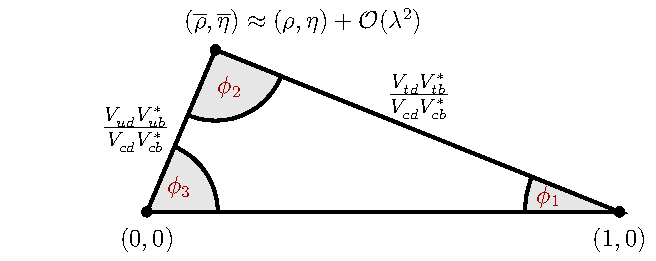
\includegraphics[scale=1]{texfig/UT_Triangle}
	\captionsetup{width=0.8\linewidth}
\caption{Unitarni trikotnik s parametri $\lambda,~\eta,~\rho$ and $A$ (slednji ni prikazan), ki predstavljajo proste parametre matrike CKM. Trikotnik je prikazan v Wolfensteinovi parametrizaciji \cite{PhysRevLett.51.1945}.}
\label{fig:ut_si}
\end{figure}

Procesi, ki jih "studiramo v tej analizi, so tesno povezani z elementom $V_{ub}$ matrike CKM, saj le-ta opisuje prehode kvarkov $b \to u$. Od vseh elementov je absolutna vrednost tega elementa najmanj"sa, relativna napaka pa najve"cja, zato meritve iz tega podro"cja potencialno omogo"cajo najve"cjo izbolj"savo. Tak"sni prehodi kvarkov so prisotni v ne-"carobnih (t.j. brez kvarkov $c$) semileptonskih razpadih mezonov $B$ oblike 
\begin{equation}
B^+ \to X_u^0 \ell^+ \nu_\ell,
\end{equation}
kjer $X_u^0$ predstavlja ne-"carobne mezone, $\ell$ pa je eden od nabitih leptonov. Frekvenco razpadov, ki je tesno povezana z elementom $V_{ub}$, opi"semo z ena"cbo
\begin{equation}
\mathrm{d} \Gamma \propto G_F^2 \vert V_{ub} \vert ^2 \vert L^\mu \langle X_u \vert \bar u \gamma_u \frac{1}{2} (1-\gamma_5) b \vert B \rangle \vert ^2,
\end{equation}
kjer $G_F$ predstavlja Fermijevo konstanto, $L^\mu$ leptonski tok, izraz v Diracovih oklepajih pa hadronski tok. V tak"snih prehodih $\vert V_{ub} \vert ^2$ predstavlja verjetnost za prehod $b \to u$.

Meritev elementa $V_{ub}$ je mo"zna na ekskluziven in inkluziven na"cin, kjer pri prvi metodi opravljamo meritve v specifi"cno definirana kon"cna stanja, kot na primer $B \to \pi \ell \nu$, pri drugi metodi pa opravljamo meritev v skupno kon"cno stanje oblike $B \to X_u \ell \nu$. Obe metodi potekata preko razli"cnih pristopov in se soo"cata z razli"cnimi te"zavami, kar pomeni, da sta oba kon"cna rezultata v ve"cji meri neodvisna. Obe meritvi imata tudi zelo podobno natan"cnost, medtem ko se srednja vrednost le deloma ujema. Rezultata se razlikujeta s signifikanco $3\sigma$, kar predstavlja ve"cjo te"zavo znotraj podro"cja. Trenutni svetovni povpre"cji \cite{Amhis:2016xyh} ekskluzivne (iz razpadov $B^0 \to \pi^- \ell^+ \nu$) in inkluzivne meritve (GGOU kolaboracija \cite{Gambino:2007rp}) sta
\begin{align}
&\vert V_{ub} \vert_{\mathrm{e.}} = \left(3,65 \pm 0,09 \pm 0,11\right)\E{-3},\\
&\vert V_{ub} \vert_{\mathrm{i.}}^{\mathrm{GGOU}} = \left(4,52 \pm 0,15~{}^{+0,11}_{-0,14}\right)\E{-3},
\end{align}
kjer prva in druga napaka predstavljata eksperimentalno in teoretsko napako. Rezultati inkluzivnih meritev so praviloma ve"cjih vrednosti kot rezultati ekskluzivnih. Razlogov za neujemanje je lahko ve"c, od nepoznanih napak pri eksperimentu ali teoriji, do prispevkov nove fizike.

V tej analizi se osredoto"camo na enega od mo"znih razlogov za zgoraj omenjeno neujemanje, konkretneje za razpad \decayb, ki je strukturno precej podoben razpadu $B \to \pi \ell \nu$ za razliko produkcije para kvarkov $s \bar s$ ki se potem hadronizira v nove delce, kot prikazuje Slika \ref{feynman_si}. V inkluzivnih meritvah ne-"carobnih semileptonskih razpadov mezonov $B$ se standardno uporablja $K$-veto, t.j. selekcija, kjer zahtevamo, da v kon"cnem stanju nimamo mezonov $K$ (sestava $q \bar s,~q \in [u,d]$), poznanih tudi pod imenom kaoni. Kaoni v kon"cnem stanju nakazujejo na pogost prehod kvarkov $b \to c \to s$, ki pa jih ho"cemo v analizah prehodov $b \to u$ zatreti. V primeru na"se analize imamo v kon"cnem stanju 2 kaona s prehodom $b \to u$, kar pomeni, da tak"sni razpadi niso upo"stevani v inkluzivnih meritvah, "ceprav bi morali biti. Cilj "studije je dolo"citi pogostost razpadov \decayb~s prehodom $b\to u$ in s tem oceniti, kak"sen potencialen efekt ima lahko neupo"stevanje teh razpadov na inkluzivno meritev elementa $V_{ub}$. V nadaljevanju bo razpad \decayb~zaradi enostavnosti zapisan kot \decaya.
\begin{figure}[H]
\centering
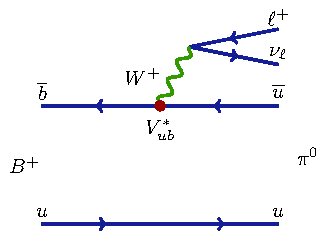
\includegraphics{texfig/B2pilnu}
\hspace{1cm}
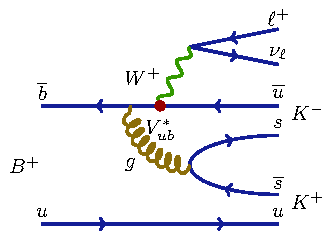
\includegraphics{texfig/B2KKlnu}
	\captionsetup{width=0.8\linewidth}
\caption{Feynmanovi diagrami za razpada $B^+ \to \pi^0 \ell^+ \nu_\ell$ (levo) in $B^+ \to K^- K^+ \ell^+ \nu_\ell$ (desno).}
\label{feynman_si}
\end{figure}

\section{Experimentalna postavitev}

Podatki, uporabljeni v tej analizi, so bili ustvarjeni pri trkih elektronov $e^-$ in pozitronov $e^+$ v pospe"sevalniku KEKB in zajeti z detektorjem Belle. Eksperiment je trajal od leta 1999 do 2010 pod okriljem znanstvene organizacije KEK v mestu Tsukuba na Japonskem. Trki delcev so se dogajali pri energiji, ki je ustrezala masi resonance $\Upsilon(4S)$, (sestava $b \bar b$). Podrobnej"si opis pospe"sevalnika in detektorja se nahaja v literaturah \cite{doi:10.1093/ptep/pts102} in \cite{ABASHIAN2002117}.

\subsection{Trkalnik KEKB}
Trkalnik KEKB je asimetri"cen trkalnik delcev $e^+e^-$, ki potujejo po obro"cih s premerom $3\e{km}$ v gru"cah. V sredi"s"cu detektorja gru"ci elektronov z energijo $8\e{GeV}$ in pozitronov z energijo $3,5\e{GeV}$ tr"cita pod kotom $22\e{mrad}$. Skupna invariantna masa trka ustreza masi resonance $\Upsilon(4S)$ 
\begin{equation}
E_{CM} = \sqrt{2E_{e^+}E_{e^-}} = m_{\Upsilon(4S)}c^2 \approx 10,58\e{GeV}.
\end{equation}
Dele"z mezonov $\Upsilon(4S)$ razpade preko zelo "cistega kanala v dva prakti"cno mirujo"ca mezona $B$ v te"zi"s"cnem sistemu, kar v tej in v podobnih analizah pogosto izkori"s"camo, saj je za"cetno stanje dobro poznano.

Trkalnik je v "casu obratovanja zajel koli"cino podatkov, ki ustreza integrirani luminoznosti $1041\e{fb^{-1}}$, od katere okoli $711\e{fb^{-1}}$ predstavlja podatke, zajete pri energiji $10,58\e{GeV}$, t.j. masi resonance $\Upsilon(4S)$. Slednja vrednost integrirane luminoznosti ustreza "stevilu $771\E{6}$ parov $B \bar B$ mezonov.

\subsection{Detektor Belle}
Detektor Belle je magnetni masni spektrometer, ki pokriva ve"cji del prostorskega kota. Njegov namen je, da detektira delce, ki se gibljejo v magnetnem polju $1,5\e{T}$ in so potomci trkov $e^+e^-$. Cilj je dolo"citi energijo in gibalno koli"cino delcev, kar dose"zemo preko detektorskih podsistemov, ki so okoli interacijske to"cke postavljeni v plasteh, kot je prikazano na Sliki \ref{fig:bdet_si}. Detektor pokriva polarni kot med $17^\circ \leq \theta \leq 150^\circ$, med tem ko je azimutni kot pokrit v celoti, kar skupaj predstavlja $92\%$ pokritost polnega prostorskega kota.

\begin{figure}[H]
	\centering
	\captionsetup{width=0.8\linewidth}
	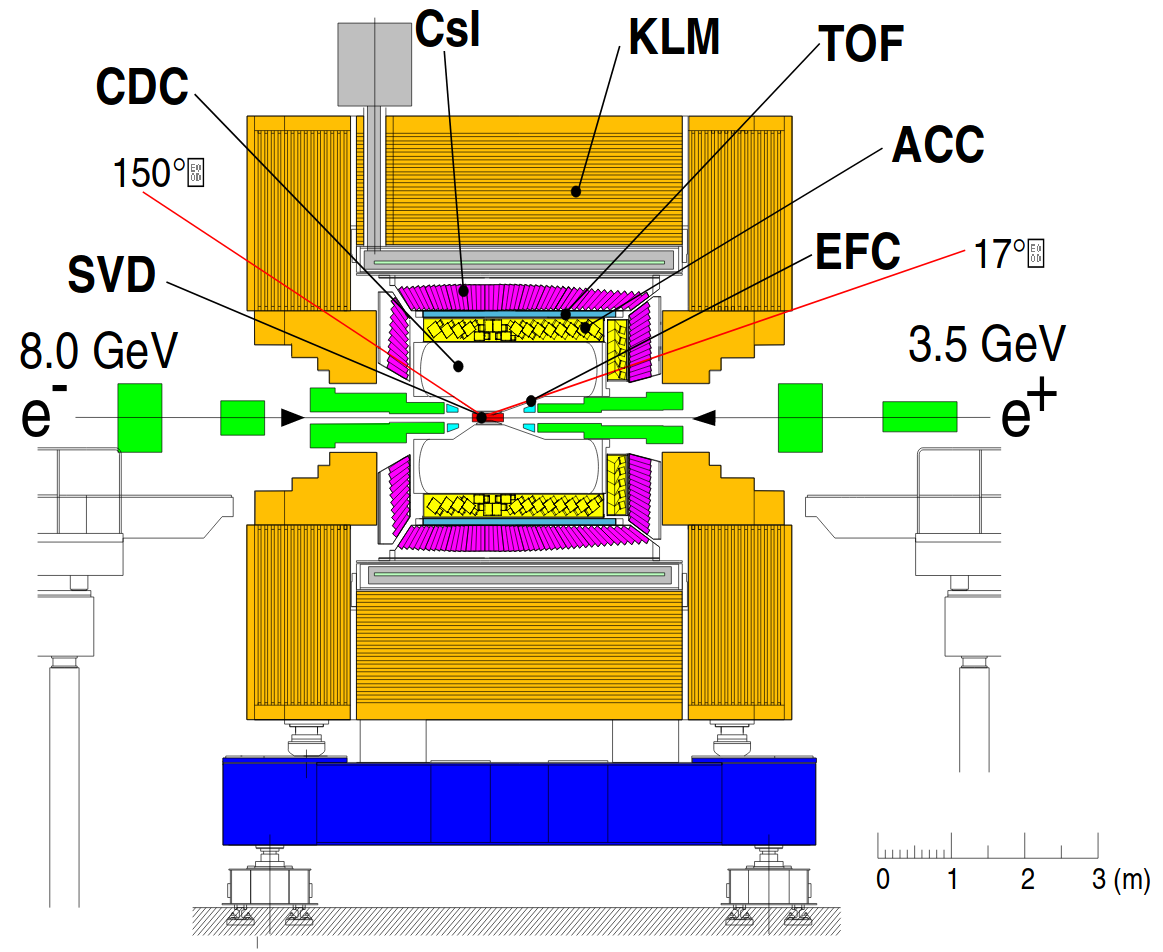
\includegraphics[width=0.8\linewidth]{fig/setup/Belle_detector}
	\caption{Shematski prikaz detektorja Belle in ustreznih podsistemov \cite{ABASHIAN2002117}.}
	\label{fig:bdet_si}
\end{figure}

\subsubsection{Silikonski  detektor verteksov}
Silikonski detektor verteksov je postavljen najbli"zje interakcijski to"cki. Sestavljen je iz dvostranskih silikonskih detektorjev, ki podajajo 2D informacijo o prehodih nabitih delcev z natan"cnostjo okoli $100\e{\mu m}$. To nam omogo"ca dolo"citev to"ck razpada (verteksov) kratko-"zive"cih delcev.

\subsubsection{Osrednja potovalna komora}
Osrednja potovalna komora je sestavljena iz mnogih "zic, napeljanih skozi skrbno izbrano me"sanico plina. Komora tako meri sledi nabitih delcev, ki potujejo skozi magnetno polje v detektorju. Preko sledi lahko dolo"cimo informacijo o gibalni koli"cini delca, hkrati pa v obmo"cju gibalne koli"cine pod $0,8\e{GeV}/c$ komora slu"zi tudi za njihovo identifikacijo.

\subsubsection{Merilec "casa preleta}
Merilec "casa preleta meri "casovno razliko od trka pa do preleta delca skozi enega od scintilatorjev tega podsistema. Namen je identifikacija delcev v obmo"cju gibalnih koli"cin $0,8\e{GeV}/c < p < 1,2\e{GeV}/c$, "se posebej kaonov $K^\pm$ in pionov $\pi^\pm$. Pri isti gibalni koli"cini zaradi razli"cnih mas delcev dobimo razli"cne "case preleta, kar lahko uporabimo za dolo"citev njihove mase. "Casovna resolucijo tega podsistema ima zgornjo mejo $100\e{ps}$.

\subsubsection{Pragovni "stevec sevanja "Cerenkova}
"Stevec sevanja "Cerenkova se prav tako uporablja za identifikacijo delcev, deluje pa v vi"sjih obmo"cjih gibalne koli"cine $1,0\e{GeV}/c < 4,0\e{GeV}/c$, kjer merilec "casa preleta ni ve"c zadosten. Silikatni aerogel, ki z dobro dolo"cenim lomnim koli"cnikom predstavlja osrednjo strukturo podsistema, seva svetlobo "Cerenkova, "ce ga preletijo delci, ki se gibljejo hitreje od svetlobne hitrosti v tej snovi. Pragovni "stevec deluje na osnovi, da prelet la"zjih delcev povzro"ci sevanje "Cerenkova, prelet te"zjih delcev pa ne.

\subsubsection{Elektromagnetni kalorimeter}
Elektromagnetni kalorimeter slu"zi za detekcijo delcev, ki interagirajo elektromagnetno. Karakteristi"cno so to elektroni in fotoni. Z njim lahko izmerimo pozicijo in energijo delca, ko zadane kalorimeter. Ko elektroni ali fotoni zadenejo kristalne celice kalorimetra, povzro"cijo t.i. elektromagnetni tu"s, medtem ko drugi, te"zji delci, ne interagirajo na enak na"cin in v kalorimetru pustijo le majhen dele"z energije. Energijska lo"cljivost kalorimetra je pribli"zno $1,7\%$.

\subsubsection{Detektor mezonov $K_L^0$ in mionov}
Za elektromagnetnim kalorimetrom, na drugi strani magnetnega jedra, je postavljen detektor mezonov $K_L^0$ in mionov za gibalno koli"cino ve"cjo od $0,6\e{GeV}/c$. Ti delci so visoko penetrirajo"ci, saj lahko preletijo vse do sedaj opisane podsisteme. Prvi so nevtralni in jih lahko dolo"cimo preko hadronske interakcije v detektorju in preko manjkajo"ce nabite sledi, medtem ko so drugi nabiti in jih identificiramo "ze samo z njihovo prisotnostjo.

\section{Analizni postopek}
Analizni postopek je dolo"cen na podlagi simuliranih podatkov, oziroma Monte Carlo (MC) simulacije. Ta nam omogo"ca, da na podlagi teoreti"cnega modela razpadov dobro opi"semo realnost, dodatno pa nam je na voljo "resnica", kot na primer generirane lastnosti delcev in njihova identiteta, ki je bila dolo"cena pri generaciji podatkov.

Za pripravo analiznega postopka imamo na voljo $6-10\times$ ve"c podatkov kot jih je izmerjenih, s "cimer pove"camo natan"cnost analiznih korakov in zmanj"samo mo"znost statisti"cnih fluktuacij.

Poleg signalnega razpada \decayb~v "studiji rekonstruiramo tudi kontrolni razpad $B^+ \to \bar D {}^0 \ell^+ \nu,~\bar D{}^0 \to K^+K^-$. Drugi ima enako kon"cno stanje kot prvi, le da poteka preko prehoda kvarkov $b \to c$ in ne $b \to u$, kot pri prvem razpadu. Uspe"sno jih lahko lo"cimo preko invariantne mase dveh kaonov, ki je v primeru kontrolnega razpada zelo omejena na obmo"cje okoli mase mezona $D^0$, v primeru signalnega razpada pa je razporejena po celotnem obmo"cju, kot prikazuje Slika \ref{fig:mKK_si}.

\begin{figure}[H]
	\centering
	\captionsetup{width=0.8\linewidth}
	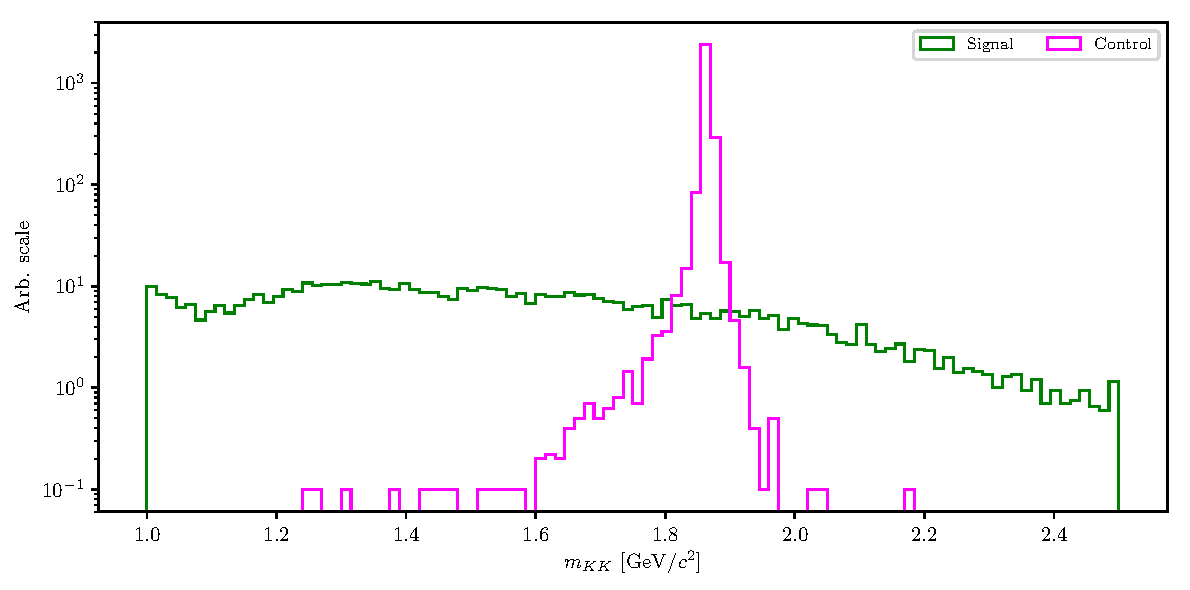
\includegraphics[width=\linewidth]{fig/mKK_si}
	\caption{Porazdelitev mase dveh kaonov ($m_{KK}$) za signalni in kontrolni razpad. Porazdelitev $m_{KK}$ kontrolnega razpada je prisotna samo v obmo"cju mase mezona $D^0$, medtem ko je porazdelitev $m_{KK}$ signalnega razpada prisotna po "sir"sem obmo"cju.}
	\label{fig:mKK_si}
\end{figure}

\subsection{Rekonstrukcija razpada}

Postopek rekonstrukcije se pri"cne z izbiro dolgo-"zive"cih stabilnih delcev, ki so v na"sem primeru elektroni $e^\pm$, mioni $\mu^\pm$ ter kaoni $K^\pm$. Vsi so nabiti in v detektorju pustijo sled. Nevtrino $\nu$ je nevtralen in interagira le preko "sibke interakcije, zato jih s tak"snim detektorjem ne moremo opaziti, kar predstavlja manjkajo"co energijo in gibalno koli"cino v dogodku trka $e^+e^-$.

Selekcija poteka na podlagi rezov spremenljivk, kjer je izbrano obmo"cje dolo"ceno na podlagi optimizacije metrike FOM (ang. \textit{figure of merit}), definirane kot 

\begin{equation}
FOM = \frac{N_S}{\sqrt{N_S + N_O}},
\end{equation}
kjer $N_S$ predstavlja "stevilo pravilno rekonstruiranih kandidatov (signal), $N_O$ pa "stevilo nepravilno rekonstruiranih kandidatov.

Povzeta selekcija dolgo-"zive"cih stabilnih delcev je
\begin{itemize}
\item elektroni: $\vert d_0 \vert < 0,1\e{cm}, \vert z_0 \vert < 1,5\e{cm},~p_{CMS} \in [0,4,\,2,6]\e{GeV}/c,~PID_e > 0,9$,
\item mioni: $\vert d_0 \vert < 0,1\e{cm},~\vert z_0 \vert < 1,5\e{cm},~p_{CMS} \in [0,6,\,2,6]\e{GeV}/c,~PID_\mu > 0,97$,
\item kaoni: $\vert d_0 \vert < 0,15\e{cm},~\vert z_0 \vert < 1,5\e{cm},~p_{CMS} \in [0,0,\,2,5]\e{GeV}/c,~PID_{K/\pi} > 0,6$,
\end{itemize}
kjer $d_0$ in $z_0$ predstavljata vpadne parametre nabitih delcev, $p_{CMS}$ gibalno koli"cino v te"zi"s"cnem koordinatnem sistemu, $PID_e$ in $PID_\mu$ metriko identifikacije delcev za elektrone in mione, $PID_{K/\pi}$ pa metriko separacije med kaoni in pioni.

Iz izbranih kandidatov nato naredimo kombinacije $Y = KKe,~KK\mu$, ki slu"zijo kot kandidati mezonov $B$, z izjemo manjkajo"cih nevtrinov. Na podlagi dejstva, da je detektor Belle hermeti"cno zaprt in pokriva ve"cino prostorskega kota, in da dobro poznamo za"cetno stanje $\Upsilon(4S)$, lahko dolo"cimo "cetverec manjkajo"ce (ang. \textit{missing}) gibalne koli"cine kot
\begin{align}
\mathrm{p}_{miss} &= \mathrm{p}_{\Upsilon(4S)} - \sum_i^{\mathrm{Dogodek}}\left(E_i,\,\vec{p}_i \right),\\
\label{eq:ROEloop_si}
\mathrm{p}_{miss} &= \mathrm{p}_{\Upsilon(4S)} - \left(\mathrm{p}_{Y} -\sum_i^{\mathrm{ROE}}\left(E_i,\,\vec{p}_i \right)\right),
\end{align}
kjer $\mathrm{p}$ predstavlja "cetverec gibalne koli"cine, indeks $i$ te"ce po vseh delcih znotraj mno"zice, ROE (ang. \textit{rest of event}) pa predstavlja podmno"zico celotnega dogodka trka $e^+e^-$, ki vsebuje vse delce, ki niso bili uporabljeni v rekonstrukciji kandidata $Y$.

Tudi na tej stopnji je prisotnih veliko napa"cnih kombinacij kandidatov $Y$, zato po enakem postopku optimiziramo nadaljnjo selekcijo

\begin{itemize}
\item mezoni $B$: 
\begin{itemize}
	\item $P(\chi^2, NDF) > 6,0\E{-3}$, 
	\item $\vert \cos \theta_{BY} \vert < 1,05$,  
	\item $m_{miss}^2 < 0,975\e{GeV}/c^2$, 
	\item $5,1\e{GeV}/c^2 < M_{BC} < 5,295\e{GeV}/c^2$, 
	\item $-1,0\e{GeV} < \Delta E < 1,3\e{GeV},$
\end{itemize} 
\end{itemize}
kjer $P(\chi^2, NDF)$ predstavlja kvaliteto rekonstrukcije verteksa mezona $B$, $m_{miss}^2$ pa invariantno maso "cetverca manjkajo"ce gibalne koli"cine v dogodku. Ostali izrazi za $\cos \theta_{BY}$, $M_{BC}$ in $\Delta E$ so
\begin{align}
%TODO fix p in Mbc
\cos \left(\theta_{BY}\right) &= \frac{2E_BE_Y - m_B^2 - m_Y^2}{2\vert \vec{p}_B \vert \vert \vec{p}_Y\vert},\\
M_{BC} &= \sqrt{\left(E_{CMS}/2\right)^2 - \vert \vec{p}_B \vert^2},\\
\Delta E &= E_B - E_{CMS}/2
\end{align}
in po vrsti predstavljajo kot med nominalnim ($B$) in rekonstruiranim ($Y$) mezonom $B$, maso, vezano na energijo "zarka v te"zi"s"cnem koordinatnem sistemu, in razliko energije kandidata in polovice te"zi"s"cne energije $E_{CMS}$. Za pravilne kombinacije mezonov $B$ se porazdelitev po $\cos \left(\theta_{BY}\right)$ nahaja na intervalu $[-1, 1]$, porazdelitvi $M_{BC}$ in $\Delta E$ pa imata vrh okoli $m_B$ in $0\e{GeV}$, kjer $m_B$ predstavlja nominalno maso mezona $B$.

Potrebno je omeniti, da so v posameznem dogodku lahko prisotni tako nevtralni kot nabiti delci, ki ne prihajajo neposredno iz trka, temve"c so lahko bodisi produkti sekundarnih interakcij v detektorju, bodisi delci, ki izhajajo iz ozadja na ra"cun raznih interakcij "zarkov med potovanjem po obro"cih pospe"sevalnika. Tak"sne delce je potrebno odstraniti iz En. (\ref{eq:ROEloop_si}), "cemur pravimo "ci"s"cenje dogodka. V tej analizi je bilo opravljeno temeljito "ci"s"cenje tako nevtralnih kot nabitih delcev, ki je terjalo razli"cne pristope. V ta namen so bile uporabljene metode strojnega u"cenja za prepoznavanje tak"snih ne"zelenih delcev. Slika \ref{fig:roe_cleanup_si} prikazuje primerjavo med o"ci"s"cenim in neo"ci"s"cenim dogodkom, kjer primerjamo porazdelitvi \varss.

\begin{figure}[H]
	\centering
	\captionsetup{width=0.8\linewidth}
	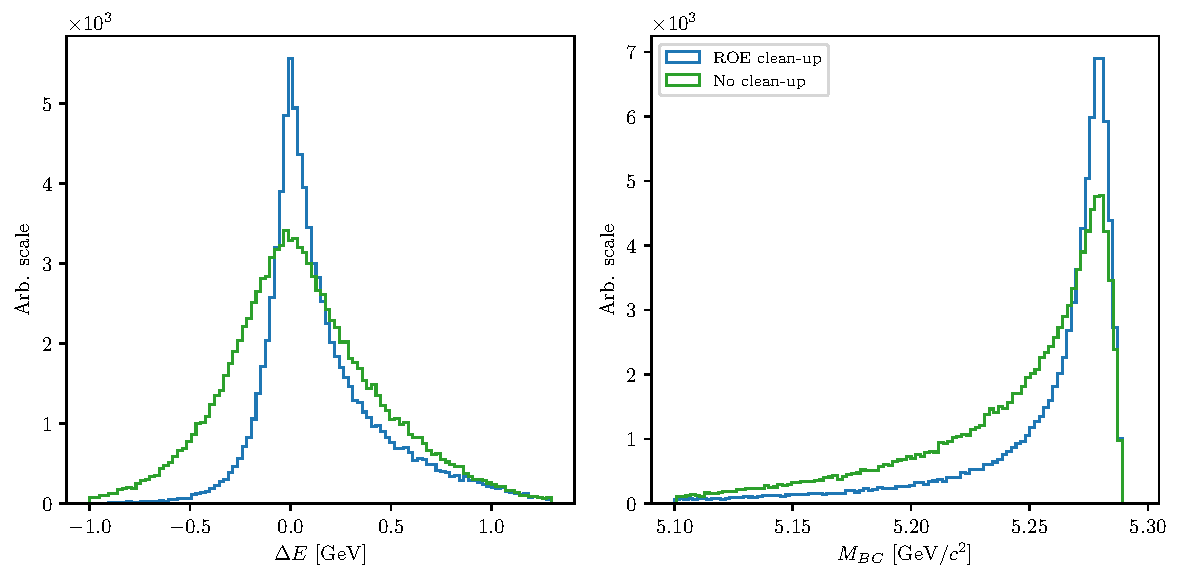
\includegraphics[width=\linewidth]{fig/roe_opt_si}
	\caption{Primerjava o"ci"s"cenega in neo"ci"s"cenega dogodka za porazdelitvi \varss. Porazdelitve iz o"ci"s"cenega dogodka so bolj ostre in predstavljajo bolj"so mo"znost za lo"citev od ozadja.}
	\label{fig:roe_cleanup_si}
\end{figure}

\subsection{Odstranjevanje ozadja}

Ozadje v tak"sni analizi predstavljajo napa"cne kombinacije razpadne verige signalnega kandidata. Napa"cno kombinacijo lahko predstavlja napa"cna kombinatorika ali pa primer kon"cnega stanja drugih razpadnih kanalov, ki posnema kon"cno stanje signalnega razpada. Tak"sne kombinacije v splo"snem nimajo enakih lastnosti kot signalne, zato sku"samo najti na"cine, kako tak"sno ozadje odstraniti na najbolj optimalen na"cin.

Odstranjevanja ozadja se lotimo v treh korakih, v prvem koraku uporabimo enostavne reze na invariantni masi kaonskega para, saj pri"cakujemo, da veliko parov $KK$ pride iz resonancam podobnih struktur, kot na primer $\phi \to KK$ ali $D^0 \to KK$, kjer za slednjo "ze vemo, da je prisotna v kontrolnem razpadu. Prav tako se lahko zgodi, da je eden od pionov napa"cno identificiran kot kaon in tako dobimo vrh porazdelitve, ki je zamaknjen za razliko mas masnih hipotez. Slika X prikazuje vse reze, ki jih uporabimo za odstranjevanje omenjenih kandidatov, in so
\begin{itemize}
\item signalni razpad: $\vert m_{KK} - m_{\phi} \vert > \Delta_\phi$, $\vert m_{KK} - m_{D^0} \vert > \Delta_{D^0}$, $\vert m_{K\pi} - m_{D^0} \vert > \Delta_{D^0}$,
\item kontrolni razpad: $\vert m_{KK} - m_{D^0} \vert < \Delta_{D^0}$, $\vert m_{K\pi} - m_{D^0} \vert > \Delta_{D^0}$,
\end{itemize}
kjer $m_{KK}$ predstavlja invariantno maso kaonskega para $KK$, $m_{K\pi}$ pa invariantno maso kaonskega para $KK$, kjer je bila masa kaona, katerega naboj je nasproten naboju $B$ mezona, zamenjana z maso delca $\pi$. Ostali parametri so $m_\phi \approx 1.019\e{GeV}/c^2$, $m_{D^0} \approx 1.864\e{GeV}/c^2$, $\Delta_\phi \approx 8\E{-3}\e{GeV}/c^2$ in $\Delta_{D^0} \approx 1.5\E{-2}\e{GeV}/c^2$. V primeru "studije kontrolnega razpada se osredoto"cimo na ozko okno okoli mase mezona $D^0$. 

V drugem koraku se lotimo odstranjevanja t.i. kontinuumskega ozadja, kjer kandidati prihajajo iz procesov $e^+e^- \to q \bar q,~q\in[u, d, s, c]$. Poslu"zimo se metod strojnega u"cenja, ki prepoznajo kandidate iz kontinuumskih procesov od signalnih kandidatov. Za ta namen potrebujemo spremenljivke, ki opisujejo sferi"cne momente fizikalnih dogodkov, saj so le-ti zelo razli"cni med procesi $e^+e^- \to q \bar q$ in $e^+e^- \to B \bar B$.

V tretjem koraku se na podoben na"cin lotimo odstranjevanja ostalih kandidatov iz procesov $e^+e^- \to B \bar B$, za kar uporabimo vse ostale lastnosti kandidatov, razen \varss, ker le-te potrebujemo za lu"s"cenje "stevila signalnih kandidatov. Pri odstranjevanju ozadja te vrste uporabimo posebno metodo strojnega u"cenja, ki ohranja obliko porazdelitve spremenljivke $M_{BC}$ za ozadje, kar prepre"cuje, da bi optimizacija preoblikovala obliko porazdelitve ozadja v tisto od signala.

Kot v prej"snjih optimizacijah optimiziramo metriko FOM za odstranjevanje ozadja v drugem in tretjem koraku. Kon"cni vzorec za signalni razpad je prikazan na Sliki \ref{fig:opt_uBB_si}, za kontrolni razpad pa na Sliki \ref{fig:onres_control_si}.

\begin{figure}[H]
	\centering
	\captionsetup{width=0.8\linewidth}
	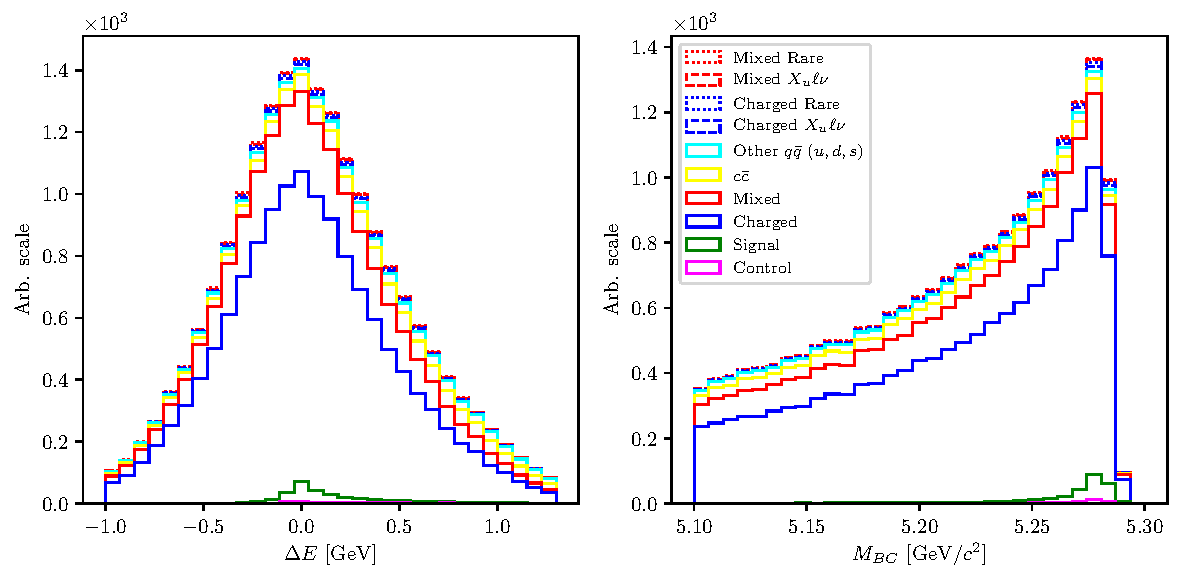
\includegraphics[width=\linewidth]{fig/opt_uBB_si}
	\caption{Porazdelitvi spremenljivk \varss~za kon"cni signalni vzorec.}
	\label{fig:opt_uBB_si}
\end{figure}

\begin{figure}[H]
	\centering
	\captionsetup{width=0.8\linewidth}
	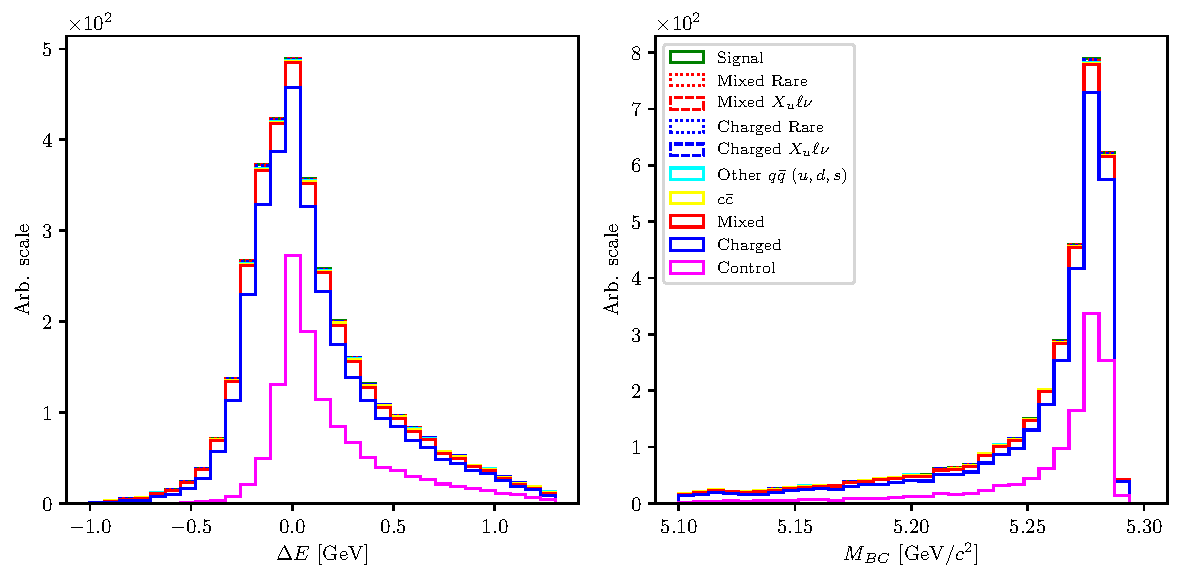
\includegraphics[width=\linewidth]{fig/onres_control_si}
	\caption{Porazdelitvi spremenljivk \varss~za kon"cni kontrolni vzorec.}
	\label{fig:onres_control_si}
\end{figure}

\subsection{Lu"s"cenje fizikalnih parametrov}

Po selekciji kon"cnega vzorca lahko za"cnemo lu"s"citi fizikalne parametre iz podatkov. Za to uporabimo orodje RooFit \cite{verkerke2006roofit}, ki nam omogo"ca, da teoreti"cni model prilagodimo izmerjenim podatkom, in na tak na"cin dolo"cimo fizikalne parametre, ki jih i"s"cemo. Na podlagi MC vzorca dolo"cimo porazdelitve za kandidate signalne kategorije in ve"cih tipov ozadja. Te porazdelitve slu"zijo kot predloge, ki jih ustrezno se"stejemo skupaj, da dobimo teoreti"cen model, ki dobro opi"se podatke.

Vsaka predloga je predstavljena kot 2-dimenzionalen histogram v spremenljivkah \varss, in sicer v $19\times 19$ razredih v zgoraj definiranem obmo"cju. Predloge posameznih kategorij so si med seboj razli"cne, kar programu omogo"ca, da z visoko verjetnostjo pravilno dolo"ci prispevke posameznih komponent.

Lu"s"cenja parametrov se lotimo z metodo najve"cje zanesljivosti (ang. \textit{maximum likelihood method}), saj nam omogo"ca zanesljivej"se rezultate, ko so signalni vzorci majhni, kot v na"sem primeru. Za vsakega od 10 vzorcev MC podatkov izvr"simo prilagajanje v namen preverjanja metode, na koncu pa enako ponovimo "se na pravih podatkih. V nadaljevanju so prikazani rezultati prilagajanja za signalni in kontrolni razpad.

\subsubsection{Kontrolni razpad}
Fizikalne parametre v primeru kontrolnega razpada izlu"s"cimo v ozkem oknu okoli mase mezona $D^0$. Pri postopku lu"s"cenja uporabimo naslednje predloge
\begin{itemize}
\item kontrolni razpad,
\item signalni razpad,
\item kontinuumsko ozadje,
\item ozadje razpada $B\to D^* \ell \nu,~D^0 \to K^+K^-$,
\item ostalo $B \bar B$ ozadje.
\end{itemize}

Slika \ref{fig:cs_fit_data_si} prikazuje primer prilagajanja predlog izmerjenim podatkom, Slika \ref{fig:cs_global_si} pa rezultate lu"s"cenja na vseh MC podatkih in na pravih podatkih. "Stevilo kandidatov kontrolnega razpada na podlagi lu"s"cenja je

\begin{table}[H]
	\centering
	\begin{tabular}{l|c|c}
		& $N^{MC}$ & $N^{\mathrm{podatki}}$ \\
		\toprule
		$\ell = e$ ali $\mu$ & $1182 \pm 11$ & $1187 \pm 44$\\
		$\ell = e$ & $591 \pm 8$ & $583 \pm 28$ \\
		$\ell = \mu$ & $592 \pm 7$ & $613 \pm 30$\\
		\bottomrule
	\end{tabular}
	\captionsetup{width=0.8\linewidth}
	\caption{Rezultati lu"s"cenja "stevila kontrolnih kandidatov za razli"cna kon"cna leptonska stanja.}
	\label{tab:cs_fit_yield_si}
\end{table}

\begin{figure}[H]
	\centering
	\captionsetup{width=0.8\linewidth}
	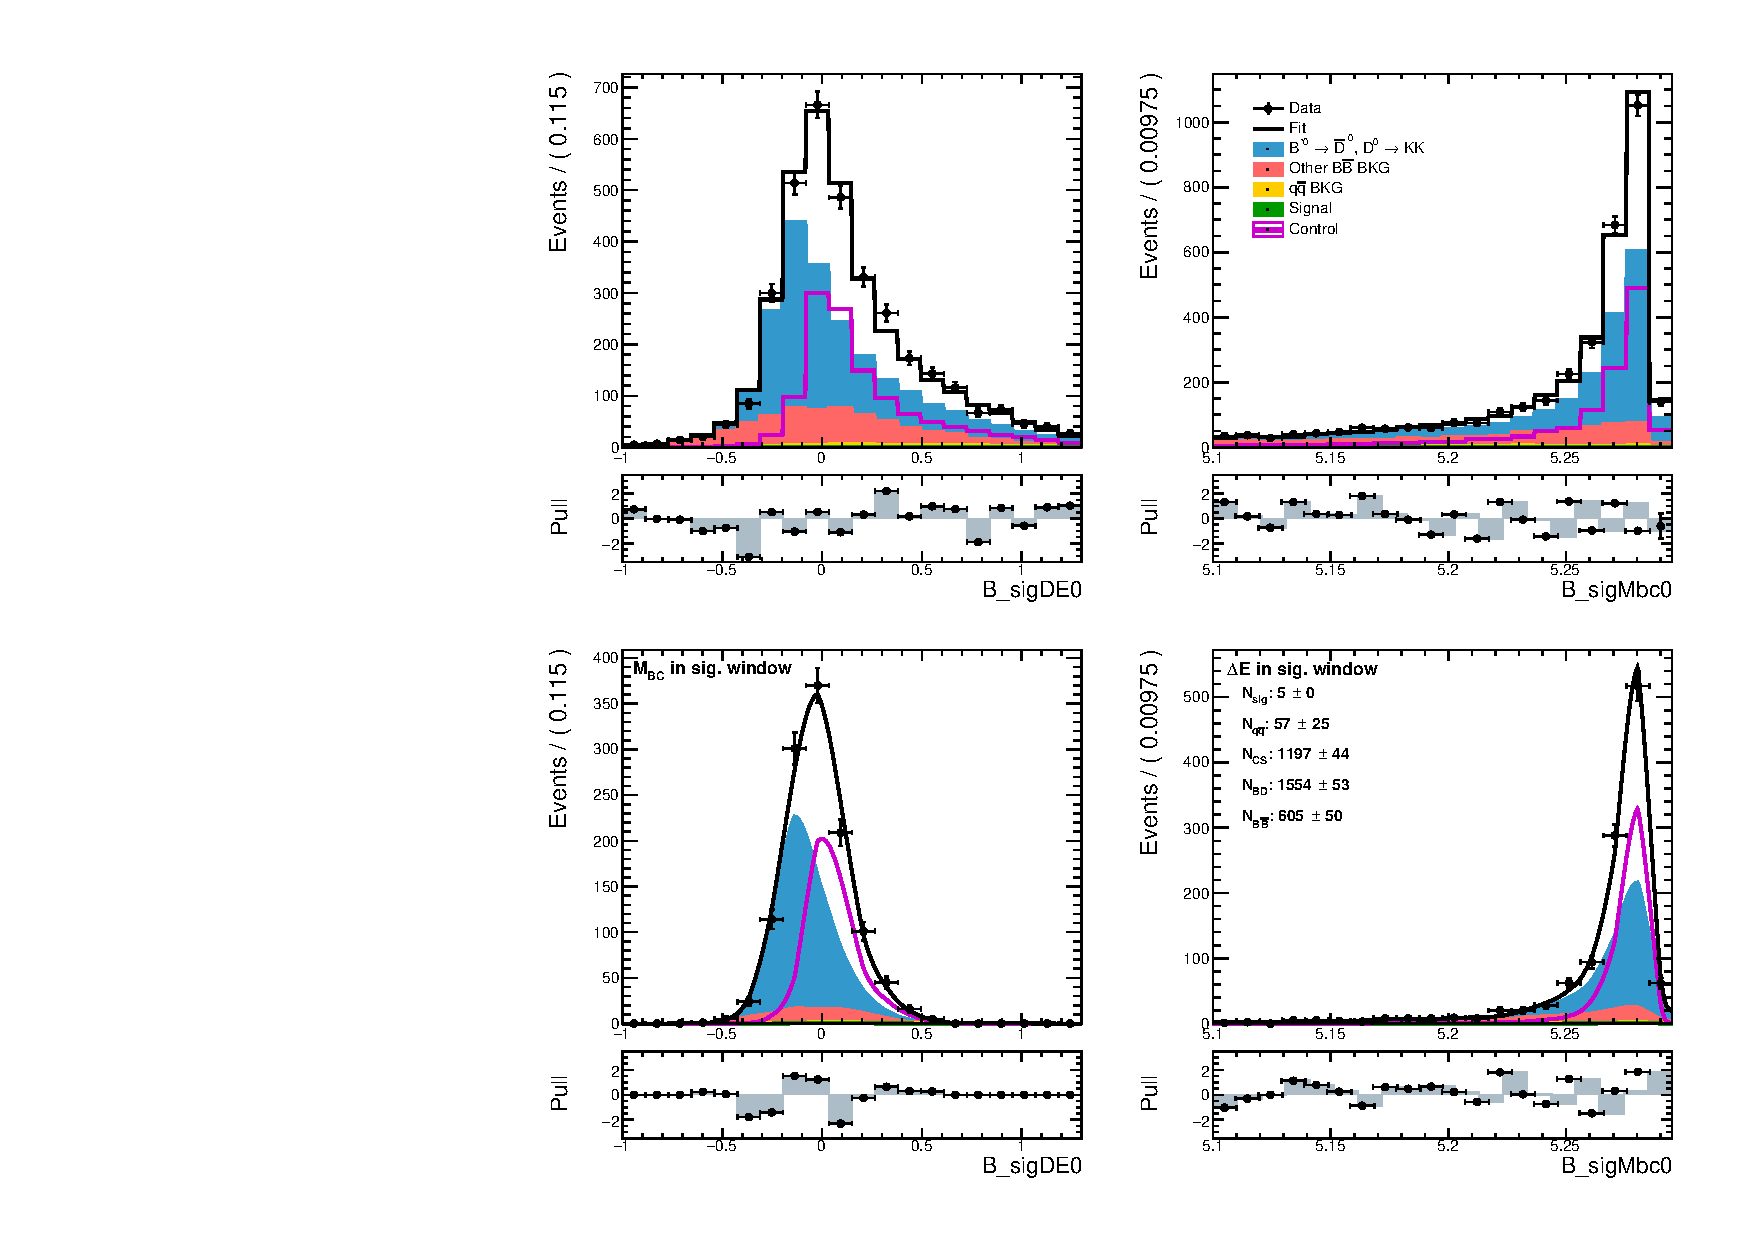
\includegraphics[width=\linewidth]{fig/cs_fit_data}
	\caption{Primer lu"s"cenja "stevila kontrolnih kandidatov na pravih podatkih. Lev stolpec prikazuje $M_{BC}$, desni pa $\Delta E$, medtem ko zgornja vrstica prikazuje porazdelitvi na celotnem definiranem obmo"cju, spodnja pa projekcija na ozko okno okoli vrha signalne porazdelitve.}
	\label{fig:cs_fit_data_si}
\end{figure}

\begin{figure}[H]
	\centering
	\captionsetup{width=0.8\linewidth}
	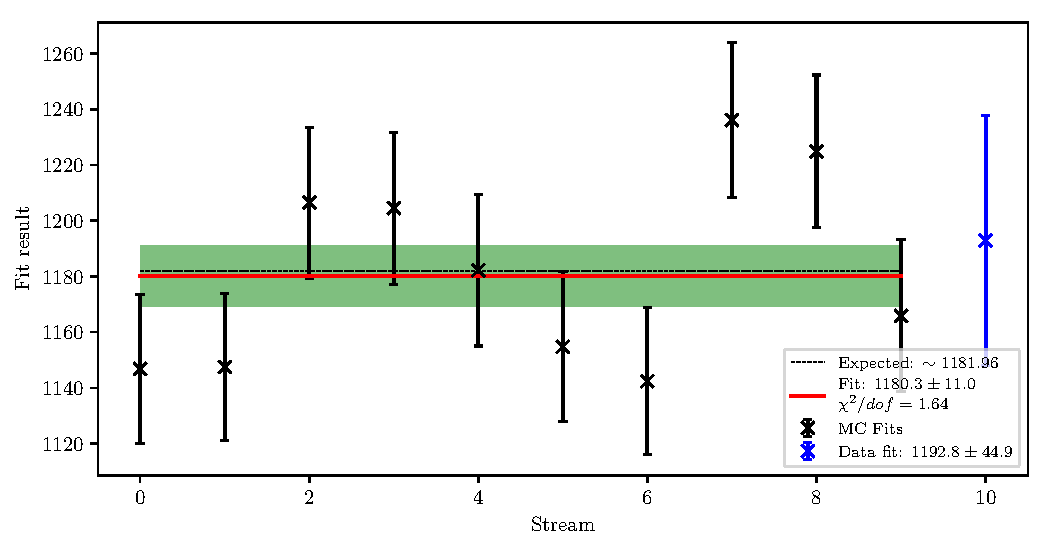
\includegraphics[width=\linewidth]{fig/cs_global}
	\caption{"Stevilo kontrolnih kandidatov za vseh 10 vzorcev MC podatkov in njihovo ute"zeno povpre"cje, ter za izmerjene podatke.}
	\label{fig:cs_global_si}
\end{figure}

Pri lu"s"cenju parametrov na pravih podatkih smo uporabili dodatno informacijo, in sicer meritev razpada $B\to D^* \ell \nu,~D^0 \to K^+K^-$ \cite{Amhis:2016xyh,tanabashi2018review}, ki smo jo uporabili v obliki omejitve vrednosti razmerja "stevila kandidatov omenjenega ter kontrolnega razpada. Na podlagi kon"cnega "stevila kandidatov kontrolnega razpada $N$ lahko dolo"cimo tudi razvejitveno razmerje, ki je dolo"ceno kot
\begin{align}
\mathcal{B} &= \frac{N \times \epsilon_{MC} \times \rho_{PID}}{2N_{B\bar B}},
\label{eq:br_data_si}
\end{align}
kjer $\epsilon_{MC}$ predstavlja izkoristek kontrolnega razpada, dolo"cenega na MC vzorcu, $\rho_{PID}$ je korekcijski faktor na ra"cun razlike identifikacij nabitih delcev na MC in na pravih podatkih, $N_{B\bar B}$ pa je izmerjeno "stevilo generiranih parov mezonov $B$. Razvejitveno razmerje lahko dolo"cimo tako na podatkih kot na MC vzorcu, rezultati obeh pa so prikazani na Sliki \ref{fig:br_plot_si}. Rezultati so konsistentni s pri"cakovanimi in izmerjenimi vrednostmi, kar potrjuje zanesljivost na"se analize.

\begin{figure}[H]
	\centering
	\captionsetup{width=0.8\linewidth}
	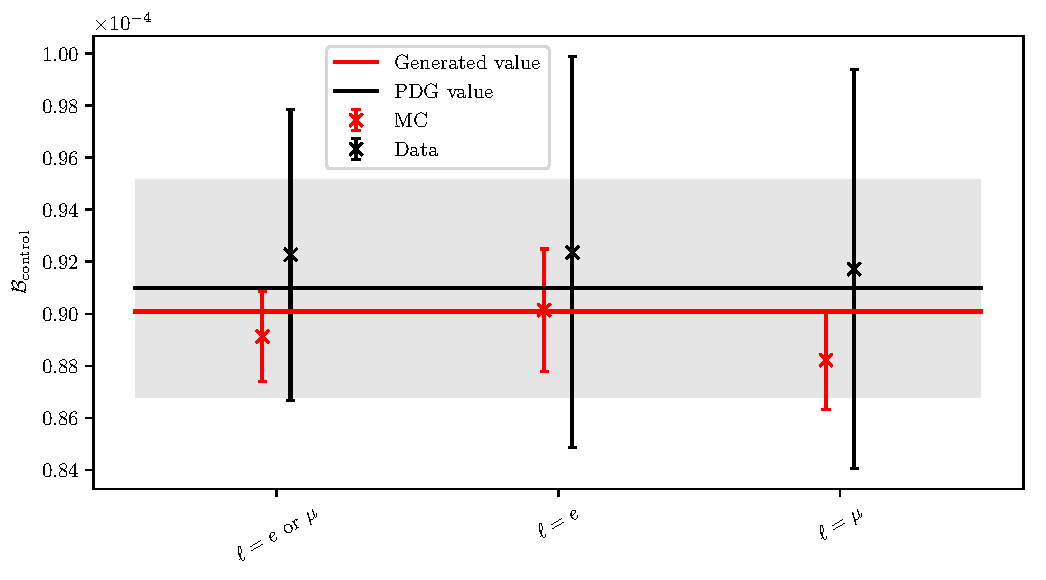
\includegraphics[width=\linewidth]{fig/br_plot}
	\caption{Rezultati meritev razvejitvenih razmerij kontrolnega razpada za MC in za podatke za razli"cna kon"cna leptonska stanja.}
	\label{fig:br_plot_si}
\end{figure}

\subsubsection{Signalni razpad}

Rezultati prilagajanja MC in pravim podatkov za kontrolni razpad potrjujejo konsistentnost na"sega analiznega postopka, tako da jih lahko ponovimo "se na signalnem razpadu. V tem primeru smo uporabili naslednje predloge
\begin{itemize}
	\item signalni razpad,
	\item kontinuumsko ozadje,
	\item dobro poznana ozadja
	\begin{itemize}
		\item $C_0:~B^+ \to \bar{D} {}^0 \ell^+ \nu,~D^0 \to K^-K^+$ (kontrolni razpad),
		\item $C_1:~B \to \bar{D} {}^* \ell^+ \nu,~D^0 \to K^-K^+$,
		\item $C_2:~B \to \bar{D} {}^{(*)} \ell^+ \nu,~D^0 \to K^-\pi^+$,
		\item $C_3:~B \to \bar{D} {}^{(*)} \ell^+ \nu,~D^0 \to K^-K^+\pi^0,~K^-\pi^+\pi^0$,
		\item $C_4:~B \to \bar{D} {}{(*)} \ell^+ \nu,~D^0 \to K^-\ell^+\nu$,
		\item $C_5:~B^0 \to D^{(*)-} \ell^+ \nu,~D^+ \to K^-K^+\pi^+,~K^-\pi^+\pi^+$,
		\item $C_6:~$ ostali $B \to \bar D {}^{(*)} \ell^+ \nu$ razpadi,
	\end{itemize}
	\item ostalo $B \bar B$ ozadje.
\end{itemize}
V primeru dobro poznanih razpadov zopet uporabimo informacije o najnovej"sih meritvah in jih uporabimo za omejitev "stevila kandidatov posamezne kategorije. Pri prilagajanju predlog pravim podatkom smo uporabili kontrolni razpad za kalibracijo "stevila parov mezonov $B$. Slika \ref{fig:sig_datafit_si} prikazuje primer prilagajanja predlog izmerjenim podatkom, Slika \ref{fig:sig_global_si} pa prikazuje rezultate lu"s"cenja na vseh MC in na pravih podatkih skupaj. "Stevila kandidatov signalnega razpada in ostalih prispevkov na podlagi lu"s"cenja so

\begin{table}[H]
	\centering
	\begin{tabular}{l|l}
		Kategorija & "Stevilo kandidatov \\
		\toprule
		Signal & $491 \pm 86$ \\
		$q \bar q$ ozadje & $ 2385 \pm 181 $ \\
		$C_0$ & $ 45 \pm 7 $ \\
		$C_1$ & $ 57 \pm 8 $\\
		$C_2$ & $ 69 \pm 9 $ \\
		$C_3$ & $ 907 \pm 57 $ \\
		$C_4$ & $ 178 \pm 16 $ \\
		$C_5$ & $ 224 \pm 18 $ \\
		$C_6$ & $ 322 \pm 108 $ \\
		Ostalo $B \bar B$ ozadje & $ 16382 \pm 247 $ \\
		\bottomrule
	\end{tabular}
	\captionsetup{width=.8\linewidth}
	\caption{"Stevila kandidatov vseh prispevkov, dolo"cenih z lu"s"cenjem na signalnem vzorcu.}
	\label{tab:sig_yields_si}
\end{table}

\begin{figure}[H]
	\centering
	\captionsetup{width=0.8\linewidth}
	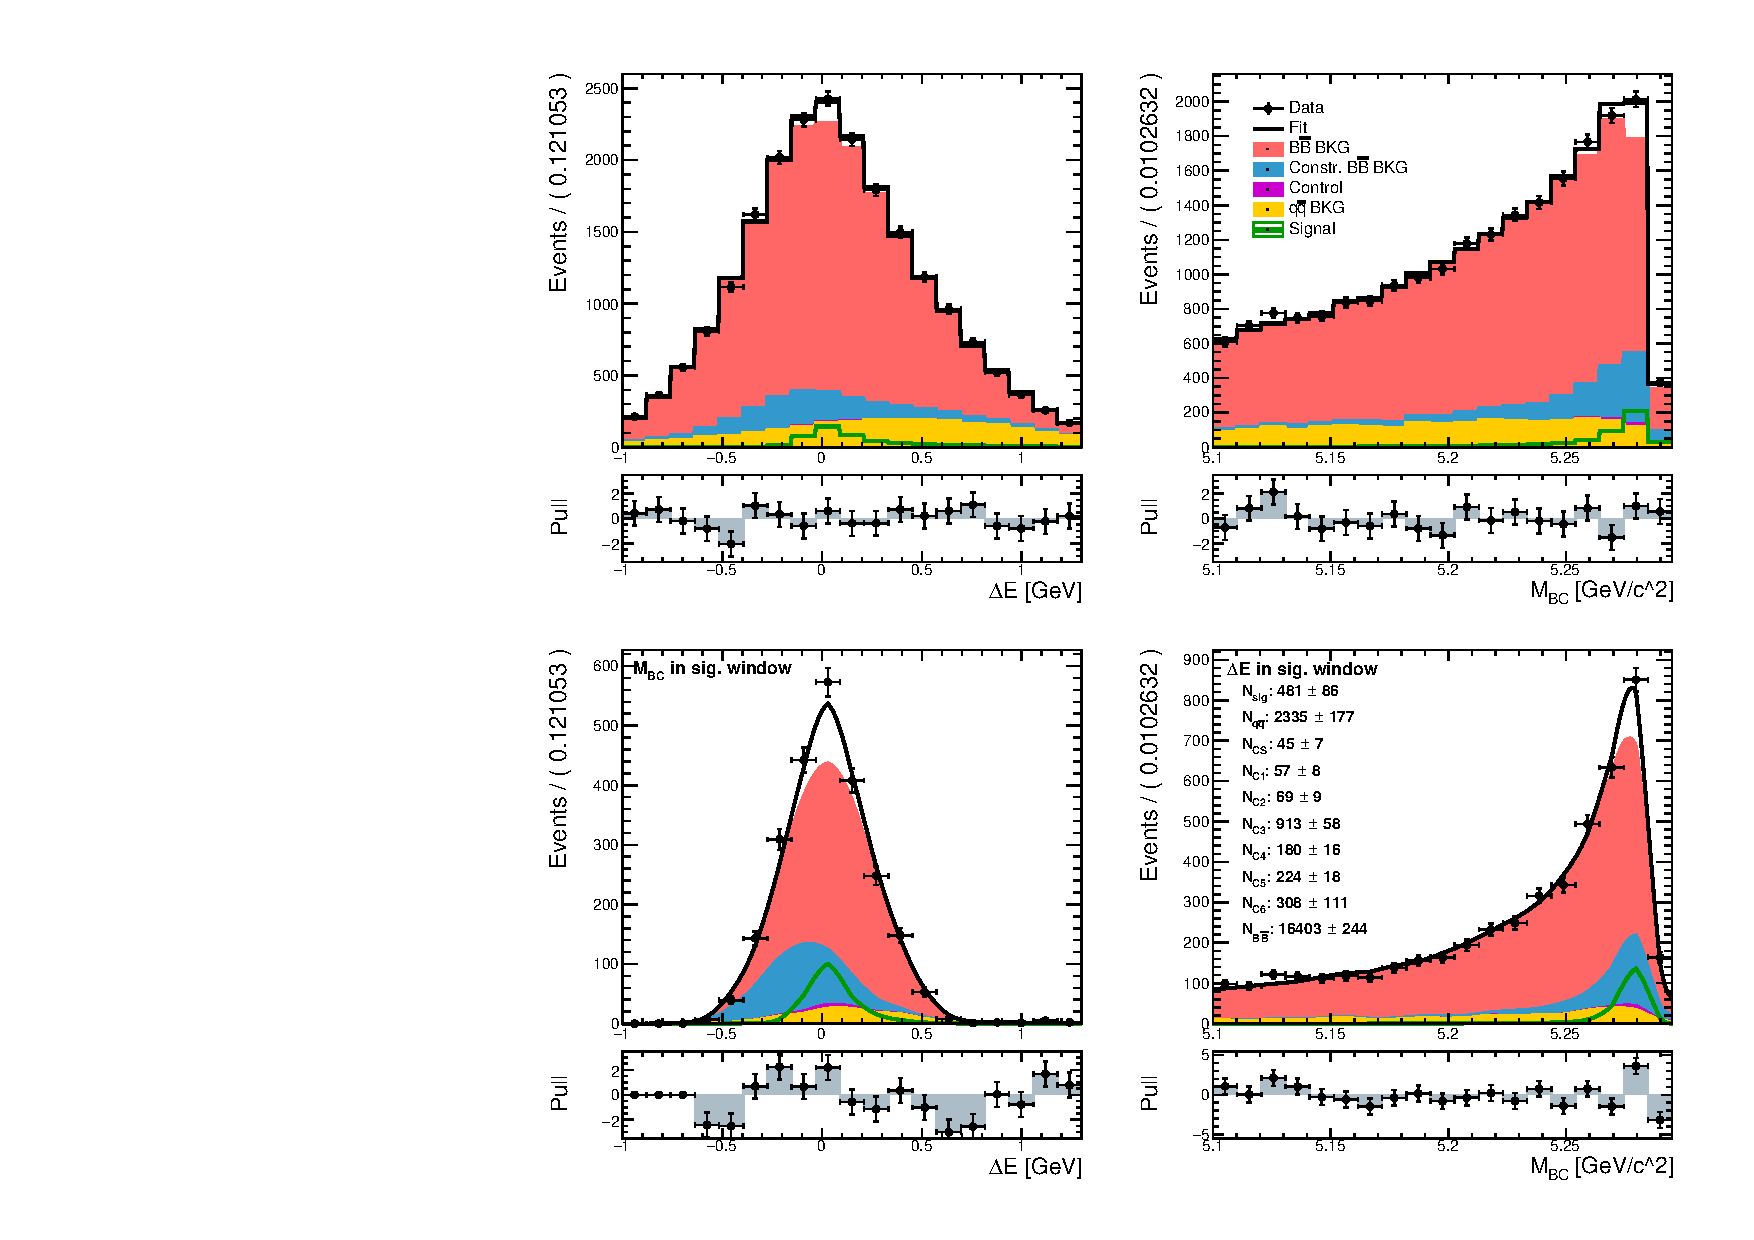
\includegraphics[width=\linewidth]{fig/sig_fit_data}
	\caption{Primer lu"s"cenja "stevila signalnih kandidatov na podatkih. Lev stolpec prikazuje $M_{BC}$, desni pa $\Delta E$, medtem ko zgornja vrstica prikazuje porazdelitvi na celotnem definiranem obmo"cju, spodnja pa projekcija na ozko okno okoli vrha signalne porazdelitve.}
	\label{fig:sig_datafit_si}
\end{figure}

\begin{figure}[H]
	\centering
	\captionsetup{width=0.8\linewidth}
	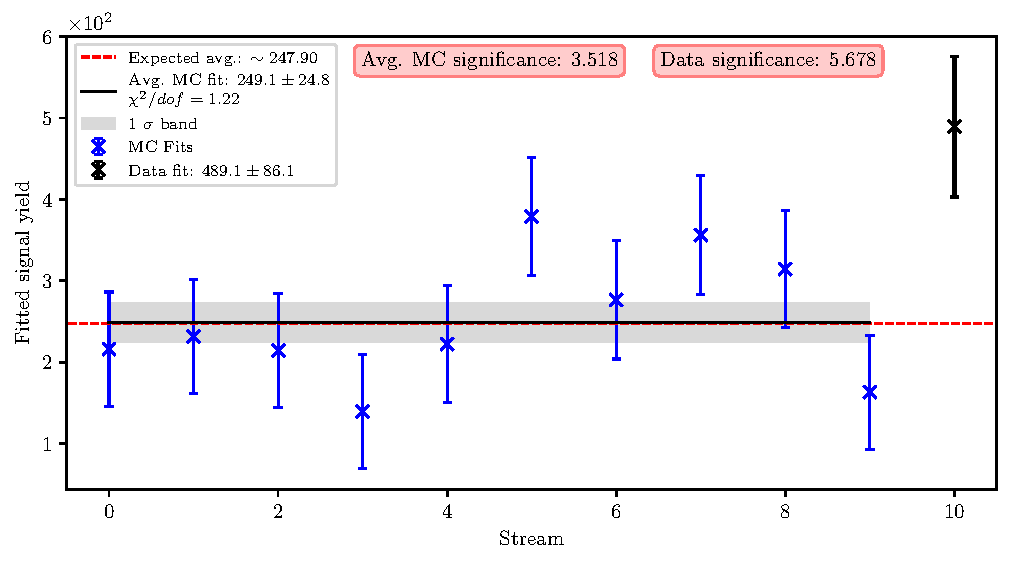
\includegraphics[width=\linewidth]{fig/sig_global}
	\caption{"Stevilo kontrolnih kandidatov za vseh 10 vzorcev MC podatkov in njihovo ute"zeno povpre"cje, ter za izmerjene podatke.}
	\label{fig:sig_global_si}
\end{figure}

Tabela \ref{tab:br_result_sig_si} prikazuje vrednosti razvejitvenega razmerja za signalni razpad na MC in na pravih podatkih. V vseh primerih je rezultat prikazan le s statistično napako.

\begin{table}[H]
	\centering
	\begin{tabular}{l|c|c|c}
		& $\mathcal{B}_{GEN}~[\times 10^{-5}]$ & $\mathcal{B}^{MC}~[\times 10^{-5}]$ & $\mathcal{B}^{\mathrm{podatki}}~[\times 10^{-5}]$ \\
		\toprule
		$\ell = e$ ali $\mu$ & $1.57$ & $1.55 \pm 0.15$ & $3.04 \pm 0.51$\\
		\bottomrule
	\end{tabular}
	\captionsetup{width=.8\linewidth}
	\caption{Vrednost razvejitvenega razmerja signalnega razpada za MC in za podatke.}
\label{tab:br_result_sig_si}
\end{table}

\section{Sistematske negotovosti}

Sistematske negotovosti vstopijo v analizo zaradi razli"cnih razlogov, bodisi zaradi poznanih razlik med MC in med podatki, bodisi zaradi pomanjkljivosti pristopov v posameznih analiznih korakih. Nekatere negotovosti so splo"sne in v naprej pripravljene za vse analize znotraj posameznih eksperimentov, medtem ko so druge specifi"cne za vsako posamezno analizo in jih je potrebno temeljito preveriti. 

\subsection{Posamezni prispevki}

\subsubsection{Identifikacija delcev}
Selekcija delcev na podlagi njihove metrike identifikacije (PID) se razlikuje na MC in na podatkih. Razlike so bile izra"cunane v za to namenjenih "studijah znotraj kolaboracije. V tej analizi obravnavamo kaone, elektrone in mione, kon"cna sistematska negotovost za obravnavan izvor pa je
\begin{equation}
\sigma_{\mathrm{sis}}^{\mathrm{PID}} = 10,\quad \delta_{\mathrm{sis}}^{\mathrm{PID}} = 2.0\%,
\end{equation}

\subsubsection{Pristranskost postopka lu"s"cenja parametrov}
Zanesljivost postopka lu"s"cenja parametrov je odvisna od kvalitete predlog posameznih kategorij, saj so si lahko nekatere predloge v nekaterih pogledih podobne in lahko na tak na"cin pod- ali precenimo njihovo amplitudo (ang. \textit{bias}). Na podlagi dveh razli"cnih "studij ocenimo, da je sistematska negotovost kon"cne vrednosti na ra"cun izbire postopka lu"s"cenja parametrov enaka
\begin{equation}
\sigma_{\mathrm{sis}}^{\mathrm{bias}} = {}^{+7}_{-10},\quad \delta_{\mathrm{sis}}^{\mathrm{bias}} = {}^{+1.5\%}_{-2.0\%}.
\end{equation}

\subsubsection{Omejitev dobro poznanega ozadja}
V postopku lu"s"cenja parametrov uporabimo informacijo o meritvah dobro poznanih razpadnih kanalov za omejitev "stevila kandidatov v obliki Gaussove porazdelitve. Te omejitve niso del statisti"cne napake, ampak spadajo med prispevke sistematskih negotovosti. V tej "studiji smo ta prispevek lo"cili in dolo"cili vrednost te sistematske negotovosti, ki je enaka
\begin{align}
\sigma_{\mathrm{sis}}^{gaus} = 26,\quad \delta_{\mathrm{sis}}^{GC} = 5.3\%,
\end{align}

\subsubsection{Zamik in raz"siritev porazdelitve $\Delta E$}

Da bi MC porazdelitve bolje pribli"zali tistim iz pravih podatkov, sta v tej analizi bila predstavljena dva nova parametra, ki na porazdelitev $\Delta E$ delujeta kot zamik in raz"siritev. Centralna vrednost parametrov in intervali zanesljivosti so bili dolo"ceni kot
\begin{itemize}
	\item Raz"siritev: $40_{-17}^{+15}\e{MeV}$,
	\item Zamik: $6_{-6}^{+4.6}\e{MeV}$.
\end{itemize}
Sistematska negotovost kon"cnega rezultata na podlagi izbire teh dveh parametrov je tako
\begin{align}
\sigma_{\mathrm{sis}}^{\mathrm{raz.}} = {}^{+41}_{-33},&\quad \delta_{\mathrm{sis}}^{\mathrm{raz.}} = {}^{+8.3\%}_{-6.7\%}, \\
\sigma_{\mathrm{sis}}^{\mathrm{zam.}} = {}^{+41}_{-31},&\quad \delta_{\mathrm{sis}}^{\mathrm{zam.}} = {}^{+9.3\%}_{-8.0\%}.
\end{align}

\subsubsection{Vpliv velikosti MC vzorca}
V analizi uporabimo porazdelitve na podlagi MC vzorca in na podlagi teh porazdelitev zgradimo cel analizni postopek. MC vzorec je kon"cne velikosti in lahko statisti"cno fluktuira, kar lahko spremeni vrednost rezultatov. Na podlagi simulacij statisti"cnih fluktuacij dolo"cimo prispevek sistematske negotovosti
\begin{equation}
\sigma_{\mathrm{sis}}^{MC} = 26,\quad \delta_{\mathrm{sis}}^{MC} = 2.4\%.
\end{equation}


\subsubsection{Izkoristek multivariatnih postopkov}
Kot re"ceno, kontrolni razpad slu"zi namenu, da preverimo analizne korake na MC in na izmerjenih podatkih, brez da bi pri tem tvegali pristranskost pri signalnem razpadu. Na tak na"cin lahko preverimo tudi kompleksnej"se postopke, ki vklju"cujejo strojno u"cenje, tako da primerjamo razmerje "stevila kandidatov kontrolnega razpada na MC in na podatkih za vsak posamezen korak aplikacije multivariatnih postopkov. Sistematska negotovost tega prispevka je dolo"cena kot standardna deviacija teh razmerij, s kon"cno vrednostjo
\begin{equation}
\sigma_{\mathrm{sis.}}^{\mathrm{MVA}} = 5,\quad\sigma_{\mathrm{sis.}}^{\mathrm{MVA}} = 1.0\%.
\end{equation}

\subsubsection{Negotovost signalnega modela}
V tej analizi je za generacijo signalnih kandidatov bil uporabljen model \texttt{ISGW2} \cite{Scora:1995ty}, za katerega je znano, da se njegova napoved slab"se ujema z meritvami. Na podlagi te zanesljivosti je postopek analize bil zastavljen "cimbolj neodvisno od modela. Kvalitativno je to sistematsko negotovost na ra"cun odvisnosti modela te"zko oceniti, zato so v ta namen bili uporabljeni trije dodatni modeli, katerih lastnosti so precej razli"cne od pri"cakovanih, in tako slu"zijo za oceno prispevka sistematske negotovosti. Prvi del prispevka prihaja na račun vpliva izbire modela na obliko \varss. Z uporabo porazdelitev, pridobljenih z omenjenimi modeli, smo dolo"cili nove vrednosti izlu"s"cenih parametrov, njihovo razliko med glavno vrednostjo pa uporabili za oceno tega dela sistematske negotovosti, ki je
\begin{equation}
\sigma_{\mathrm{sis}}^{\mathrm{mod.~obl.}} = {}^{+45}_{-39},\quad \delta_{\mathrm{sis}}^{\mathrm{mod.~obl.}} = {}^{+9.3\%}_{-8.0\%}.
\end{equation}
Drugi del prispevka določimo na podlagi povprečnega izkoristka različnih modelov. Do različnih izkoristkov lahko pride zato, ker imajo različni modeli različne lastnosti razpada, kar vpliva na učinkovistost analiznega postopka. Na podlagi razlik izkoristkov različnih modelov v primerjavi z glavnim določimo oceno tega dela sistematske negotovosti, ki je
\begin{equation}
\sigma_{\mathrm{sis}}^{\mathrm{mod.~izk.}} = {}^{+70}_{-79},\quad \delta_{\mathrm{sys}}^{\mathrm{mod.~izk.}} = {}^{+14.3\%}_{-16.2\%}.
\end{equation}
\subsection{Povzetek sistematskih negotovosti}

Tabela \ref{tab:sys_summary_si} prikazuje posamezne prispevke sistematskih negotovosti in njihovo skupno vrednost, ki je bila uporabljena pri dolo"citvi kon"cnega rezultata.

\begin{table}[H]
	\centering
	\begin{tabular}{l|l|l}
		Prispevek & $\sigma$ & $\delta~[\%]$ \\
		\toprule
		Identifikacija delcev & $10$ & $2$ \\
		Pristranskost postopka & $ {}^{+7}_{-10}$ & ${}^{+1.5}_{-2.1}$ \\
		Omejitev poznanega ozadja & $26$ & $5.3$ \\
		Zamik $\Delta E$ & ${}^{+41}_{-33}$ & ${}^{+8.3}_{-6.7}$ \\
		Raz"siritev $\Delta E$ & ${}^{+41}_{-31}$ & ${}^{+8.4}_{-6.3}$ \\
		Velikost MC vzorca & $26$ & $5.3$ \\
		Izkoristek multiv. postopkov & $5$ & $1.0$\\
		Oblika signalnih modelov & ${}^{+45}_{-39}$ & ${}^{+9.3}_{-8.0}$ \\
		Izkoristek signalnih modelov & ${}^{+70}_{-79}$ & ${}^{+14.3}_{-16.2}$ \\
		\midrule
		Skupaj & ${} ^{+109}_{-107}$ & ${}^{+22.2}_{-21.9}$ \\
		\bottomrule
	\end{tabular}
	\captionsetup{width=0.8\linewidth}
	\caption{Povzetek sistematskih negotovosti te analize.}
	\label{tab:sys_summary_si}
\end{table}

\section{Končni rezultat in zaključek}
Delo predstavlja prvo meritev razpada \decayb. Z upoštevanjem vseh sistematičnih negotovosti lahko določimo končni rezultat za razvejitveno razmerje razpada, ki znaša
\begin{equation}
\mathcal{B}(B^+ \to K^+ K^- \ell^+ \nu) = (3.04 \pm 0.51 \pm {}^{+0.67}_{-0.66})\E{-5},
\end{equation}
kjer prva napaka predstavlja statistično negotovost, druga pa sistematično. Statistična signifikanca signala v tem delu je enaka $6.3\sigma$, skupna signifikanca pa $4.6\sigma$, s čimer meritev pridobi status dokaza za signalni razpad \decayb. 

\end{otherlanguage}
